\documentclass{book}
\usepackage[a4paper,top=2.5cm,bottom=2.5cm,left=2.5cm,right=2.5cm]{geometry}
\usepackage{makeidx}
\usepackage{natbib}
\usepackage{graphicx}
\usepackage{multicol}
\usepackage{float}
\usepackage{listings}
\usepackage{color}
\usepackage{ifthen}
\usepackage[table]{xcolor}
\usepackage{textcomp}
\usepackage{alltt}
\usepackage{ifpdf}
\ifpdf
\usepackage[pdftex,
            pagebackref=true,
            colorlinks=true,
            linkcolor=blue,
            unicode
           ]{hyperref}
\else
\usepackage[ps2pdf,
            pagebackref=true,
            colorlinks=true,
            linkcolor=blue,
            unicode
           ]{hyperref}
\usepackage{pspicture}
\fi
\usepackage[utf8]{inputenc}
\usepackage{mathptmx}
\usepackage[scaled=.90]{helvet}
\usepackage{courier}
\usepackage{sectsty}
\usepackage{amssymb}
\usepackage[titles]{tocloft}
\usepackage{doxygen}
\lstset{language=C++,inputencoding=utf8,basicstyle=\footnotesize,breaklines=true,breakatwhitespace=true,tabsize=8,numbers=left }
\makeindex
\setcounter{tocdepth}{3}
\renewcommand{\footrulewidth}{0.4pt}
\renewcommand{\familydefault}{\sfdefault}
\hfuzz=15pt
\setlength{\emergencystretch}{15pt}
\hbadness=750
\tolerance=750
\begin{document}
\hypersetup{pageanchor=false,citecolor=blue}
\begin{titlepage}
\vspace*{7cm}
\begin{center}
{\Large Module Image }\\
\vspace*{1cm}
{\large Generated by Doxygen 1.8.1.2}\\
\vspace*{0.5cm}
{\small Tue Mar 5 2013 14:19:51}\\
\end{center}
\end{titlepage}
\clearemptydoublepage
\pagenumbering{roman}
\tableofcontents
\clearemptydoublepage
\pagenumbering{arabic}
\hypersetup{pageanchor=true,citecolor=blue}
\chapter{Class Index}
\section{Class List}
Here are the classes, structs, unions and interfaces with brief descriptions\-:\begin{DoxyCompactList}
\item\contentsline{section}{\hyperlink{structImage}{Image} }{\pageref{structImage}}{}
\item\contentsline{section}{\hyperlink{structPixel}{Pixel} }{\pageref{structPixel}}{}
\end{DoxyCompactList}

\chapter{File Index}
\section{File List}
Here is a list of all files with brief descriptions\-:\begin{DoxyCompactList}
\item\contentsline{section}{/home/antoine/\-Projets/tron-\/lif7/src/\hyperlink{Controle_8h}{Controle.\-h} \\*Module des vecteurs }{\pageref{Controle_8h}}{}
\item\contentsline{section}{/home/antoine/\-Projets/tron-\/lif7/src/\hyperlink{Grid_8h}{Grid.\-h} \\*Module des vecteurs }{\pageref{Grid_8h}}{}
\item\contentsline{section}{/home/antoine/\-Projets/tron-\/lif7/src/\hyperlink{main_8cpp}{main.\-cpp} }{\pageref{main_8cpp}}{}
\item\contentsline{section}{/home/antoine/\-Projets/tron-\/lif7/src/\hyperlink{Moto_8h}{Moto.\-h} \\*Module des Motos du jeu }{\pageref{Moto_8h}}{}
\item\contentsline{section}{/home/antoine/\-Projets/tron-\/lif7/src/\hyperlink{Mur_8h}{Mur.\-h} }{\pageref{Mur_8h}}{}
\item\contentsline{section}{/home/antoine/\-Projets/tron-\/lif7/src/\hyperlink{Vecteur2D_8c}{Vecteur2\-D.\-c} }{\pageref{Vecteur2D_8c}}{}
\item\contentsline{section}{/home/antoine/\-Projets/tron-\/lif7/src/\hyperlink{Vecteur2D_8h}{Vecteur2\-D.\-h} \\*Module des vecteurs }{\pageref{Vecteur2D_8h}}{}
\end{DoxyCompactList}

\chapter{Class Documentation}
\hypertarget{structImage}{\section{Image Struct Reference}
\label{structImage}\index{Image@{Image}}
}


{\ttfamily \#include $<$image.\-h$>$}

\subsection*{Public Attributes}
\begin{DoxyCompactItemize}
\item 
\hyperlink{structPixel}{Pixel} $\ast$ \hyperlink{structImage_aa8d8f858fa81a873f20acdb61281bfb3}{tab}
\item 
unsigned int \hyperlink{structImage_a846f530876e1296835bd6ab42a22890d}{dimx}
\item 
unsigned int \hyperlink{structImage_a02275f30d94fbc73fd8f6d594823acf4}{dimy}
\end{DoxyCompactItemize}


\subsection{Member Data Documentation}
\hypertarget{structImage_a846f530876e1296835bd6ab42a22890d}{\index{Image@{Image}!dimx@{dimx}}
\index{dimx@{dimx}!Image@{Image}}
\subsubsection[{dimx}]{\setlength{\rightskip}{0pt plus 5cm}unsigned int Image\-::dimx}}\label{structImage_a846f530876e1296835bd6ab42a22890d}
\hypertarget{structImage_a02275f30d94fbc73fd8f6d594823acf4}{\index{Image@{Image}!dimy@{dimy}}
\index{dimy@{dimy}!Image@{Image}}
\subsubsection[{dimy}]{\setlength{\rightskip}{0pt plus 5cm}unsigned int Image\-::dimy}}\label{structImage_a02275f30d94fbc73fd8f6d594823acf4}
\hypertarget{structImage_aa8d8f858fa81a873f20acdb61281bfb3}{\index{Image@{Image}!tab@{tab}}
\index{tab@{tab}!Image@{Image}}
\subsubsection[{tab}]{\setlength{\rightskip}{0pt plus 5cm}{\bf Pixel}$\ast$ Image\-::tab}}\label{structImage_aa8d8f858fa81a873f20acdb61281bfb3}


The documentation for this struct was generated from the following file\-:\begin{DoxyCompactItemize}
\item 
/home/antoine/\-L\-I\-F7\-\_\-td/src/\hyperlink{image_8h}{image.\-h}\end{DoxyCompactItemize}

\hypertarget{structPixel}{\section{Pixel Struct Reference}
\label{structPixel}\index{Pixel@{Pixel}}
}


{\ttfamily \#include $<$pixel.\-h$>$}

\subsection*{Public Attributes}
\begin{DoxyCompactItemize}
\item 
unsigned char \hyperlink{structPixel_a038ad5b3349e7548d17c5d3bec511b94}{r}
\item 
unsigned char \hyperlink{structPixel_a8407845aacf1663d9463475619911686}{g}
\item 
unsigned char \hyperlink{structPixel_a760bdf29b15433d257f119239fcff4d4}{b}
\end{DoxyCompactItemize}


\subsection{Member Data Documentation}
\hypertarget{structPixel_a760bdf29b15433d257f119239fcff4d4}{\index{Pixel@{Pixel}!b@{b}}
\index{b@{b}!Pixel@{Pixel}}
\subsubsection[{b}]{\setlength{\rightskip}{0pt plus 5cm}unsigned char Pixel\-::b}}\label{structPixel_a760bdf29b15433d257f119239fcff4d4}
\hypertarget{structPixel_a8407845aacf1663d9463475619911686}{\index{Pixel@{Pixel}!g@{g}}
\index{g@{g}!Pixel@{Pixel}}
\subsubsection[{g}]{\setlength{\rightskip}{0pt plus 5cm}unsigned char Pixel\-::g}}\label{structPixel_a8407845aacf1663d9463475619911686}
\hypertarget{structPixel_a038ad5b3349e7548d17c5d3bec511b94}{\index{Pixel@{Pixel}!r@{r}}
\index{r@{r}!Pixel@{Pixel}}
\subsubsection[{r}]{\setlength{\rightskip}{0pt plus 5cm}unsigned char Pixel\-::r}}\label{structPixel_a038ad5b3349e7548d17c5d3bec511b94}


The documentation for this struct was generated from the following file\-:\begin{DoxyCompactItemize}
\item 
/home/antoine/\-L\-I\-F7\-\_\-td/src/\hyperlink{pixel_8h}{pixel.\-h}\end{DoxyCompactItemize}

\chapter{File Documentation}
\hypertarget{image_8c}{\section{/home/antoine/\-L\-I\-F7\-\_\-td/src/image.c File Reference}
\label{image_8c}\index{/home/antoine/\-L\-I\-F7\-\_\-td/src/image.\-c@{/home/antoine/\-L\-I\-F7\-\_\-td/src/image.\-c}}
}
{\ttfamily \#include $<$stdlib.\-h$>$}\\*
{\ttfamily \#include $<$stdio.\-h$>$}\\*
{\ttfamily \#include $<$assert.\-h$>$}\\*
{\ttfamily \#include \char`\"{}image.\-h\char`\"{}}\\*
{\ttfamily \#include \char`\"{}pixel.\-h\char`\"{}}\\*
\subsection*{Functions}
\begin{DoxyCompactItemize}
\item 
void \hyperlink{image_8c_a09752f3133d816f341b8829132336043}{im\-Init} (\hyperlink{structImage}{Image} $\ast$Im, int dimx, int dimy)
\begin{DoxyCompactList}\small\item\em im\-Init initialise dimx et dimy (après vérification) de la structure \hyperlink{structImage}{Image} puis alloue le tableau de pixel dans le tas \end{DoxyCompactList}\item 
void \hyperlink{image_8c_a5c53a00ee1712cbf4236ecf8c5c34471}{im\-Libere} (\hyperlink{structImage}{Image} $\ast$Im)
\item 
\hyperlink{structImage}{Image} $\ast$ \hyperlink{image_8c_a9a91b54dbb066e5d191fb6f23316c7f4}{im\-Creer} (int dimx, int dimy)
\item 
void \hyperlink{image_8c_a0432c9a9f4a307b34549cca27df59fb6}{im\-Detruire} (\hyperlink{structImage}{Image} $\ast$$\ast$pim)
\item 
\hyperlink{structPixel}{Pixel} \hyperlink{image_8c_ae312c8b781c888ee84c25bda908a3b55}{get\-Pix} (const \hyperlink{structImage}{Image} $\ast$Im, int x, int y)
\item 
void \hyperlink{image_8c_a5547e2784de260bc57e46673adbc4121}{set\-Pix} (\hyperlink{structImage}{Image} $\ast$Im, int x, int y, const \hyperlink{structPixel}{Pixel} $\ast$couleur)
\item 
void \hyperlink{image_8c_ab37b9cd64497d1e4fb0b87a8c6fb7873}{im\-Dessine\-Rectangle} (\hyperlink{structImage}{Image} $\ast$Im, int Xmin, int Ymin, int Xmax, int Ymax, const \hyperlink{structPixel}{Pixel} $\ast$couleur)
\item 
void \hyperlink{image_8c_afe91cb0a289ff537a64ef98dd333e71f}{im\-Effacer} (\hyperlink{structImage}{Image} $\ast$Im, const \hyperlink{structPixel}{Pixel} $\ast$couleur)
\item 
void \hyperlink{image_8c_a20b9ad35b6db7bd09d7452574d04dd50}{im\-Sauver} (const \hyperlink{structImage}{Image} $\ast$p\-Im, const char filename\mbox{[}$\,$\mbox{]})
\item 
void \hyperlink{image_8c_a0a1f0b9be4b910e1cfc2648cfa9e38fd}{im\-Ouvrir} (\hyperlink{structImage}{Image} $\ast$p\-Im, const char filename\mbox{[}$\,$\mbox{]})
\item 
void \hyperlink{image_8c_afadf8ab43119d304c72e201d0d95164d}{im\-Printf} (const \hyperlink{structImage}{Image} $\ast$p\-Im)
\item 
void \hyperlink{image_8c_a8d4964490fb1a67b590ce77acd78031f}{im\-Test\-Regression} ()
\end{DoxyCompactItemize}


\subsection{Function Documentation}
\hypertarget{image_8c_ae312c8b781c888ee84c25bda908a3b55}{\index{image.\-c@{image.\-c}!get\-Pix@{get\-Pix}}
\index{get\-Pix@{get\-Pix}!image.c@{image.\-c}}
\subsubsection[{get\-Pix}]{\setlength{\rightskip}{0pt plus 5cm}{\bf Pixel} get\-Pix (
\begin{DoxyParamCaption}
\item[{const {\bf Image} $\ast$}]{Im, }
\item[{int}]{x, }
\item[{int}]{y}
\end{DoxyParamCaption}
)}}\label{image_8c_ae312c8b781c888ee84c25bda908a3b55}
\begin{DoxyVerb}getPix récupère le pixel de coordonnée (x,y) en vérifiant leur validité
\end{DoxyVerb}
 la formule pour passer de 2\-D à un tab 1\-D est pix\mbox{[}y$\ast$dimx+x\mbox{]} \hypertarget{image_8c_a9a91b54dbb066e5d191fb6f23316c7f4}{\index{image.\-c@{image.\-c}!im\-Creer@{im\-Creer}}
\index{im\-Creer@{im\-Creer}!image.c@{image.\-c}}
\subsubsection[{im\-Creer}]{\setlength{\rightskip}{0pt plus 5cm}{\bf Image}$\ast$ im\-Creer (
\begin{DoxyParamCaption}
\item[{int}]{dimx, }
\item[{int}]{dimy}
\end{DoxyParamCaption}
)}}\label{image_8c_a9a91b54dbb066e5d191fb6f23316c7f4}
im\-Creer alloue dans le tas une structure \hyperlink{structImage}{Image} puis l'initialise avec im\-Init =$>$ 2 lignes \hypertarget{image_8c_ab37b9cd64497d1e4fb0b87a8c6fb7873}{\index{image.\-c@{image.\-c}!im\-Dessine\-Rectangle@{im\-Dessine\-Rectangle}}
\index{im\-Dessine\-Rectangle@{im\-Dessine\-Rectangle}!image.c@{image.\-c}}
\subsubsection[{im\-Dessine\-Rectangle}]{\setlength{\rightskip}{0pt plus 5cm}void im\-Dessine\-Rectangle (
\begin{DoxyParamCaption}
\item[{{\bf Image} $\ast$}]{Im, }
\item[{int}]{Xmin, }
\item[{int}]{Ymin, }
\item[{int}]{Xmax, }
\item[{int}]{Ymax, }
\item[{const {\bf Pixel} $\ast$}]{couleur}
\end{DoxyParamCaption}
)}}\label{image_8c_ab37b9cd64497d1e4fb0b87a8c6fb7873}
dessine un rectangle de couleur dans l'image en utilisant set\-Pix \hypertarget{image_8c_a0432c9a9f4a307b34549cca27df59fb6}{\index{image.\-c@{image.\-c}!im\-Detruire@{im\-Detruire}}
\index{im\-Detruire@{im\-Detruire}!image.c@{image.\-c}}
\subsubsection[{im\-Detruire}]{\setlength{\rightskip}{0pt plus 5cm}void im\-Detruire (
\begin{DoxyParamCaption}
\item[{{\bf Image} $\ast$$\ast$}]{pim}
\end{DoxyParamCaption}
)}}\label{image_8c_a0432c9a9f4a307b34549cca27df59fb6}
\begin{DoxyVerb}Libere le tableau de pixel en appelant imLibere puis détruit
\end{DoxyVerb}
 la structure image \hypertarget{image_8c_afe91cb0a289ff537a64ef98dd333e71f}{\index{image.\-c@{image.\-c}!im\-Effacer@{im\-Effacer}}
\index{im\-Effacer@{im\-Effacer}!image.c@{image.\-c}}
\subsubsection[{im\-Effacer}]{\setlength{\rightskip}{0pt plus 5cm}void im\-Effacer (
\begin{DoxyParamCaption}
\item[{{\bf Image} $\ast$}]{Im, }
\item[{const {\bf Pixel} $\ast$}]{couleur}
\end{DoxyParamCaption}
)}}\label{image_8c_afe91cb0a289ff537a64ef98dd333e71f}
efface l'image en appelant im\-Dessine\-Rectangle avec le bon rectangle \hypertarget{image_8c_a09752f3133d816f341b8829132336043}{\index{image.\-c@{image.\-c}!im\-Init@{im\-Init}}
\index{im\-Init@{im\-Init}!image.c@{image.\-c}}
\subsubsection[{im\-Init}]{\setlength{\rightskip}{0pt plus 5cm}void im\-Init (
\begin{DoxyParamCaption}
\item[{{\bf Image} $\ast$}]{Im, }
\item[{int}]{dimx, }
\item[{int}]{dimy}
\end{DoxyParamCaption}
)}}\label{image_8c_a09752f3133d816f341b8829132336043}


im\-Init initialise dimx et dimy (après vérification) de la structure \hyperlink{structImage}{Image} puis alloue le tableau de pixel dans le tas 

\hypertarget{image_8c_a5c53a00ee1712cbf4236ecf8c5c34471}{\index{image.\-c@{image.\-c}!im\-Libere@{im\-Libere}}
\index{im\-Libere@{im\-Libere}!image.c@{image.\-c}}
\subsubsection[{im\-Libere}]{\setlength{\rightskip}{0pt plus 5cm}void im\-Libere (
\begin{DoxyParamCaption}
\item[{{\bf Image} $\ast$}]{Im}
\end{DoxyParamCaption}
)}}\label{image_8c_a5c53a00ee1712cbf4236ecf8c5c34471}
Libère la mémoire du tableau de pixels et met les champs dimx et dimy de la structure à 0 \hypertarget{image_8c_a0a1f0b9be4b910e1cfc2648cfa9e38fd}{\index{image.\-c@{image.\-c}!im\-Ouvrir@{im\-Ouvrir}}
\index{im\-Ouvrir@{im\-Ouvrir}!image.c@{image.\-c}}
\subsubsection[{im\-Ouvrir}]{\setlength{\rightskip}{0pt plus 5cm}void im\-Ouvrir (
\begin{DoxyParamCaption}
\item[{{\bf Image} $\ast$}]{p\-Im, }
\item[{const char}]{filename\mbox{[}$\,$\mbox{]}}
\end{DoxyParamCaption}
)}}\label{image_8c_a0a1f0b9be4b910e1cfc2648cfa9e38fd}
\hypertarget{image_8c_afadf8ab43119d304c72e201d0d95164d}{\index{image.\-c@{image.\-c}!im\-Printf@{im\-Printf}}
\index{im\-Printf@{im\-Printf}!image.c@{image.\-c}}
\subsubsection[{im\-Printf}]{\setlength{\rightskip}{0pt plus 5cm}void im\-Printf (
\begin{DoxyParamCaption}
\item[{const {\bf Image} $\ast$}]{p\-Im}
\end{DoxyParamCaption}
)}}\label{image_8c_afadf8ab43119d304c72e201d0d95164d}
\hypertarget{image_8c_a20b9ad35b6db7bd09d7452574d04dd50}{\index{image.\-c@{image.\-c}!im\-Sauver@{im\-Sauver}}
\index{im\-Sauver@{im\-Sauver}!image.c@{image.\-c}}
\subsubsection[{im\-Sauver}]{\setlength{\rightskip}{0pt plus 5cm}void im\-Sauver (
\begin{DoxyParamCaption}
\item[{const {\bf Image} $\ast$}]{p\-Im, }
\item[{const char}]{filename\mbox{[}$\,$\mbox{]}}
\end{DoxyParamCaption}
)}}\label{image_8c_a20b9ad35b6db7bd09d7452574d04dd50}
\hypertarget{image_8c_a8d4964490fb1a67b590ce77acd78031f}{\index{image.\-c@{image.\-c}!im\-Test\-Regression@{im\-Test\-Regression}}
\index{im\-Test\-Regression@{im\-Test\-Regression}!image.c@{image.\-c}}
\subsubsection[{im\-Test\-Regression}]{\setlength{\rightskip}{0pt plus 5cm}void im\-Test\-Regression (
\begin{DoxyParamCaption}
{}
\end{DoxyParamCaption}
)}}\label{image_8c_a8d4964490fb1a67b590ce77acd78031f}
\begin{DoxyVerb}Effectue tout une série de test vérifiant que le module fonctionne et que les
\end{DoxyVerb}
 champ de la structure sont conformes \hypertarget{image_8c_a5547e2784de260bc57e46673adbc4121}{\index{image.\-c@{image.\-c}!set\-Pix@{set\-Pix}}
\index{set\-Pix@{set\-Pix}!image.c@{image.\-c}}
\subsubsection[{set\-Pix}]{\setlength{\rightskip}{0pt plus 5cm}void set\-Pix (
\begin{DoxyParamCaption}
\item[{{\bf Image} $\ast$}]{Im, }
\item[{int}]{x, }
\item[{int}]{y, }
\item[{const {\bf Pixel} $\ast$}]{couleur}
\end{DoxyParamCaption}
)}}\label{image_8c_a5547e2784de260bc57e46673adbc4121}
set\-Pix modifie le pixel de coord (x,y) 
\hypertarget{image_8h}{\section{/home/antoine/\-L\-I\-F7\-\_\-td/src/image.h File Reference}
\label{image_8h}\index{/home/antoine/\-L\-I\-F7\-\_\-td/src/image.\-h@{/home/antoine/\-L\-I\-F7\-\_\-td/src/image.\-h}}
}
{\ttfamily \#include $<$stdlib.\-h$>$}\\*
{\ttfamily \#include \char`\"{}pixel.\-h\char`\"{}}\\*
{\ttfamily \#include $<$stdio.\-h$>$}\\*
\subsection*{Classes}
\begin{DoxyCompactItemize}
\item 
struct \hyperlink{structImage}{Image}
\end{DoxyCompactItemize}
\subsection*{Functions}
\begin{DoxyCompactItemize}
\item 
void \hyperlink{image_8h_a09752f3133d816f341b8829132336043}{im\-Init} (\hyperlink{structImage}{Image} $\ast$Im, int dimx, int dimy)
\begin{DoxyCompactList}\small\item\em im\-Init initialise dimx et dimy (après vérification) de la structure \hyperlink{structImage}{Image} puis alloue le tableau de pixel dans le tas \end{DoxyCompactList}\item 
void \hyperlink{image_8h_a5c53a00ee1712cbf4236ecf8c5c34471}{im\-Libere} (\hyperlink{structImage}{Image} $\ast$Im)
\item 
\hyperlink{structImage}{Image} $\ast$ \hyperlink{image_8h_a9a91b54dbb066e5d191fb6f23316c7f4}{im\-Creer} (int dimx, int dimy)
\item 
void \hyperlink{image_8h_a0432c9a9f4a307b34549cca27df59fb6}{im\-Detruire} (\hyperlink{structImage}{Image} $\ast$$\ast$pim)
\item 
\hyperlink{structPixel}{Pixel} \hyperlink{image_8h_ae312c8b781c888ee84c25bda908a3b55}{get\-Pix} (const \hyperlink{structImage}{Image} $\ast$Im, int x, int y)
\item 
void \hyperlink{image_8h_a5547e2784de260bc57e46673adbc4121}{set\-Pix} (\hyperlink{structImage}{Image} $\ast$Im, int x, int y, const \hyperlink{structPixel}{Pixel} $\ast$couleur)
\item 
void \hyperlink{image_8h_ab37b9cd64497d1e4fb0b87a8c6fb7873}{im\-Dessine\-Rectangle} (\hyperlink{structImage}{Image} $\ast$Im, int Xmin, int Ymin, int Xmax, int Ymax, const \hyperlink{structPixel}{Pixel} $\ast$couleur)
\item 
void \hyperlink{image_8h_afe91cb0a289ff537a64ef98dd333e71f}{im\-Effacer} (\hyperlink{structImage}{Image} $\ast$Im, const \hyperlink{structPixel}{Pixel} $\ast$couleur)
\item 
void \hyperlink{image_8h_a20b9ad35b6db7bd09d7452574d04dd50}{im\-Sauver} (const \hyperlink{structImage}{Image} $\ast$p\-Im, const char filename\mbox{[}$\,$\mbox{]})
\item 
void \hyperlink{image_8h_a0a1f0b9be4b910e1cfc2648cfa9e38fd}{im\-Ouvrir} (\hyperlink{structImage}{Image} $\ast$p\-Im, const char filename\mbox{[}$\,$\mbox{]})
\item 
void \hyperlink{image_8h_afadf8ab43119d304c72e201d0d95164d}{im\-Printf} (const \hyperlink{structImage}{Image} $\ast$p\-Im)
\item 
void \hyperlink{image_8h_a8d4964490fb1a67b590ce77acd78031f}{im\-Test\-Regression} ()
\end{DoxyCompactItemize}


\subsection{Function Documentation}
\hypertarget{image_8h_ae312c8b781c888ee84c25bda908a3b55}{\index{image.\-h@{image.\-h}!get\-Pix@{get\-Pix}}
\index{get\-Pix@{get\-Pix}!image.h@{image.\-h}}
\subsubsection[{get\-Pix}]{\setlength{\rightskip}{0pt plus 5cm}{\bf Pixel} get\-Pix (
\begin{DoxyParamCaption}
\item[{const {\bf Image} $\ast$}]{Im, }
\item[{int}]{x, }
\item[{int}]{y}
\end{DoxyParamCaption}
)}}\label{image_8h_ae312c8b781c888ee84c25bda908a3b55}
\begin{DoxyVerb}getPix récupère le pixel de coordonnée (x,y) en vérifiant leur validité
\end{DoxyVerb}
 la formule pour passer de 2\-D à un tab 1\-D est pix\mbox{[}y$\ast$dimx+x\mbox{]} \hypertarget{image_8h_a9a91b54dbb066e5d191fb6f23316c7f4}{\index{image.\-h@{image.\-h}!im\-Creer@{im\-Creer}}
\index{im\-Creer@{im\-Creer}!image.h@{image.\-h}}
\subsubsection[{im\-Creer}]{\setlength{\rightskip}{0pt plus 5cm}{\bf Image}$\ast$ im\-Creer (
\begin{DoxyParamCaption}
\item[{int}]{dimx, }
\item[{int}]{dimy}
\end{DoxyParamCaption}
)}}\label{image_8h_a9a91b54dbb066e5d191fb6f23316c7f4}
im\-Creer alloue dans le tas une structure \hyperlink{structImage}{Image} puis l'initialise avec im\-Init =$>$ 2 lignes \hypertarget{image_8h_ab37b9cd64497d1e4fb0b87a8c6fb7873}{\index{image.\-h@{image.\-h}!im\-Dessine\-Rectangle@{im\-Dessine\-Rectangle}}
\index{im\-Dessine\-Rectangle@{im\-Dessine\-Rectangle}!image.h@{image.\-h}}
\subsubsection[{im\-Dessine\-Rectangle}]{\setlength{\rightskip}{0pt plus 5cm}void im\-Dessine\-Rectangle (
\begin{DoxyParamCaption}
\item[{{\bf Image} $\ast$}]{Im, }
\item[{int}]{Xmin, }
\item[{int}]{Ymin, }
\item[{int}]{Xmax, }
\item[{int}]{Ymax, }
\item[{const {\bf Pixel} $\ast$}]{couleur}
\end{DoxyParamCaption}
)}}\label{image_8h_ab37b9cd64497d1e4fb0b87a8c6fb7873}
dessine un rectangle de couleur dans l'image en utilisant set\-Pix \hypertarget{image_8h_a0432c9a9f4a307b34549cca27df59fb6}{\index{image.\-h@{image.\-h}!im\-Detruire@{im\-Detruire}}
\index{im\-Detruire@{im\-Detruire}!image.h@{image.\-h}}
\subsubsection[{im\-Detruire}]{\setlength{\rightskip}{0pt plus 5cm}void im\-Detruire (
\begin{DoxyParamCaption}
\item[{{\bf Image} $\ast$$\ast$}]{pim}
\end{DoxyParamCaption}
)}}\label{image_8h_a0432c9a9f4a307b34549cca27df59fb6}
\begin{DoxyVerb}Libere le tableau de pixel en appelant imLibere puis détruit
\end{DoxyVerb}
 la structure image \hypertarget{image_8h_afe91cb0a289ff537a64ef98dd333e71f}{\index{image.\-h@{image.\-h}!im\-Effacer@{im\-Effacer}}
\index{im\-Effacer@{im\-Effacer}!image.h@{image.\-h}}
\subsubsection[{im\-Effacer}]{\setlength{\rightskip}{0pt plus 5cm}void im\-Effacer (
\begin{DoxyParamCaption}
\item[{{\bf Image} $\ast$}]{Im, }
\item[{const {\bf Pixel} $\ast$}]{couleur}
\end{DoxyParamCaption}
)}}\label{image_8h_afe91cb0a289ff537a64ef98dd333e71f}
efface l'image en appelant im\-Dessine\-Rectangle avec le bon rectangle \hypertarget{image_8h_a09752f3133d816f341b8829132336043}{\index{image.\-h@{image.\-h}!im\-Init@{im\-Init}}
\index{im\-Init@{im\-Init}!image.h@{image.\-h}}
\subsubsection[{im\-Init}]{\setlength{\rightskip}{0pt plus 5cm}void im\-Init (
\begin{DoxyParamCaption}
\item[{{\bf Image} $\ast$}]{Im, }
\item[{int}]{dimx, }
\item[{int}]{dimy}
\end{DoxyParamCaption}
)}}\label{image_8h_a09752f3133d816f341b8829132336043}


im\-Init initialise dimx et dimy (après vérification) de la structure \hyperlink{structImage}{Image} puis alloue le tableau de pixel dans le tas 

\hypertarget{image_8h_a5c53a00ee1712cbf4236ecf8c5c34471}{\index{image.\-h@{image.\-h}!im\-Libere@{im\-Libere}}
\index{im\-Libere@{im\-Libere}!image.h@{image.\-h}}
\subsubsection[{im\-Libere}]{\setlength{\rightskip}{0pt plus 5cm}void im\-Libere (
\begin{DoxyParamCaption}
\item[{{\bf Image} $\ast$}]{Im}
\end{DoxyParamCaption}
)}}\label{image_8h_a5c53a00ee1712cbf4236ecf8c5c34471}
Libère la mémoire du tableau de pixels et met les champs dimx et dimy de la structure à 0 \hypertarget{image_8h_a0a1f0b9be4b910e1cfc2648cfa9e38fd}{\index{image.\-h@{image.\-h}!im\-Ouvrir@{im\-Ouvrir}}
\index{im\-Ouvrir@{im\-Ouvrir}!image.h@{image.\-h}}
\subsubsection[{im\-Ouvrir}]{\setlength{\rightskip}{0pt plus 5cm}void im\-Ouvrir (
\begin{DoxyParamCaption}
\item[{{\bf Image} $\ast$}]{p\-Im, }
\item[{const char}]{filename\mbox{[}$\,$\mbox{]}}
\end{DoxyParamCaption}
)}}\label{image_8h_a0a1f0b9be4b910e1cfc2648cfa9e38fd}
\hypertarget{image_8h_afadf8ab43119d304c72e201d0d95164d}{\index{image.\-h@{image.\-h}!im\-Printf@{im\-Printf}}
\index{im\-Printf@{im\-Printf}!image.h@{image.\-h}}
\subsubsection[{im\-Printf}]{\setlength{\rightskip}{0pt plus 5cm}void im\-Printf (
\begin{DoxyParamCaption}
\item[{const {\bf Image} $\ast$}]{p\-Im}
\end{DoxyParamCaption}
)}}\label{image_8h_afadf8ab43119d304c72e201d0d95164d}
\hypertarget{image_8h_a20b9ad35b6db7bd09d7452574d04dd50}{\index{image.\-h@{image.\-h}!im\-Sauver@{im\-Sauver}}
\index{im\-Sauver@{im\-Sauver}!image.h@{image.\-h}}
\subsubsection[{im\-Sauver}]{\setlength{\rightskip}{0pt plus 5cm}void im\-Sauver (
\begin{DoxyParamCaption}
\item[{const {\bf Image} $\ast$}]{p\-Im, }
\item[{const char}]{filename\mbox{[}$\,$\mbox{]}}
\end{DoxyParamCaption}
)}}\label{image_8h_a20b9ad35b6db7bd09d7452574d04dd50}
\hypertarget{image_8h_a8d4964490fb1a67b590ce77acd78031f}{\index{image.\-h@{image.\-h}!im\-Test\-Regression@{im\-Test\-Regression}}
\index{im\-Test\-Regression@{im\-Test\-Regression}!image.h@{image.\-h}}
\subsubsection[{im\-Test\-Regression}]{\setlength{\rightskip}{0pt plus 5cm}void im\-Test\-Regression (
\begin{DoxyParamCaption}
{}
\end{DoxyParamCaption}
)}}\label{image_8h_a8d4964490fb1a67b590ce77acd78031f}
\begin{DoxyVerb}Effectue tout une série de test vérifiant que le module fonctionne et que les
\end{DoxyVerb}
 champ de la structure sont conformes \hypertarget{image_8h_a5547e2784de260bc57e46673adbc4121}{\index{image.\-h@{image.\-h}!set\-Pix@{set\-Pix}}
\index{set\-Pix@{set\-Pix}!image.h@{image.\-h}}
\subsubsection[{set\-Pix}]{\setlength{\rightskip}{0pt plus 5cm}void set\-Pix (
\begin{DoxyParamCaption}
\item[{{\bf Image} $\ast$}]{Im, }
\item[{int}]{x, }
\item[{int}]{y, }
\item[{const {\bf Pixel} $\ast$}]{couleur}
\end{DoxyParamCaption}
)}}\label{image_8h_a5547e2784de260bc57e46673adbc4121}
set\-Pix modifie le pixel de coord (x,y) 
\hypertarget{main_8c}{\section{Référence du fichier main.\-c}
\label{main_8c}\index{main.\-c@{main.\-c}}
}


\hyperlink{main_8c}{main.\-c}  


{\ttfamily \#include $<$stdlib.\-h$>$}\\*
{\ttfamily \#include $<$stdio.\-h$>$}\\*
{\ttfamily \#include $<$assert.\-h$>$}\\*
{\ttfamily \#include \char`\"{}Mur.\-h\char`\"{}}\\*
{\ttfamily \#include \char`\"{}Moto.\-h\char`\"{}}\\*
{\ttfamily \#include \char`\"{}Controle.\-h\char`\"{}}\\*
{\ttfamily \#include \char`\"{}Joueur.\-h\char`\"{}}\\*
{\ttfamily \#include \char`\"{}Grid.\-h\char`\"{}}\\*
{\ttfamily \#include \char`\"{}Jeu.\-h\char`\"{}}\\*
{\ttfamily \#include \char`\"{}S\-D\-L.\-h\char`\"{}}\\*
{\ttfamily \#include \char`\"{}Bonus.\-h\char`\"{}}\\*
{\ttfamily \#include \char`\"{}Constantes.\-h\char`\"{}}\\*
{\ttfamily \#include \char`\"{}Musique.\-h\char`\"{}}\\*
{\ttfamily \#include $<$time.\-h$>$}\\*
Graphe des dépendances par inclusion de main.\-c\-:
\nopagebreak
\begin{figure}[H]
\begin{center}
\leavevmode
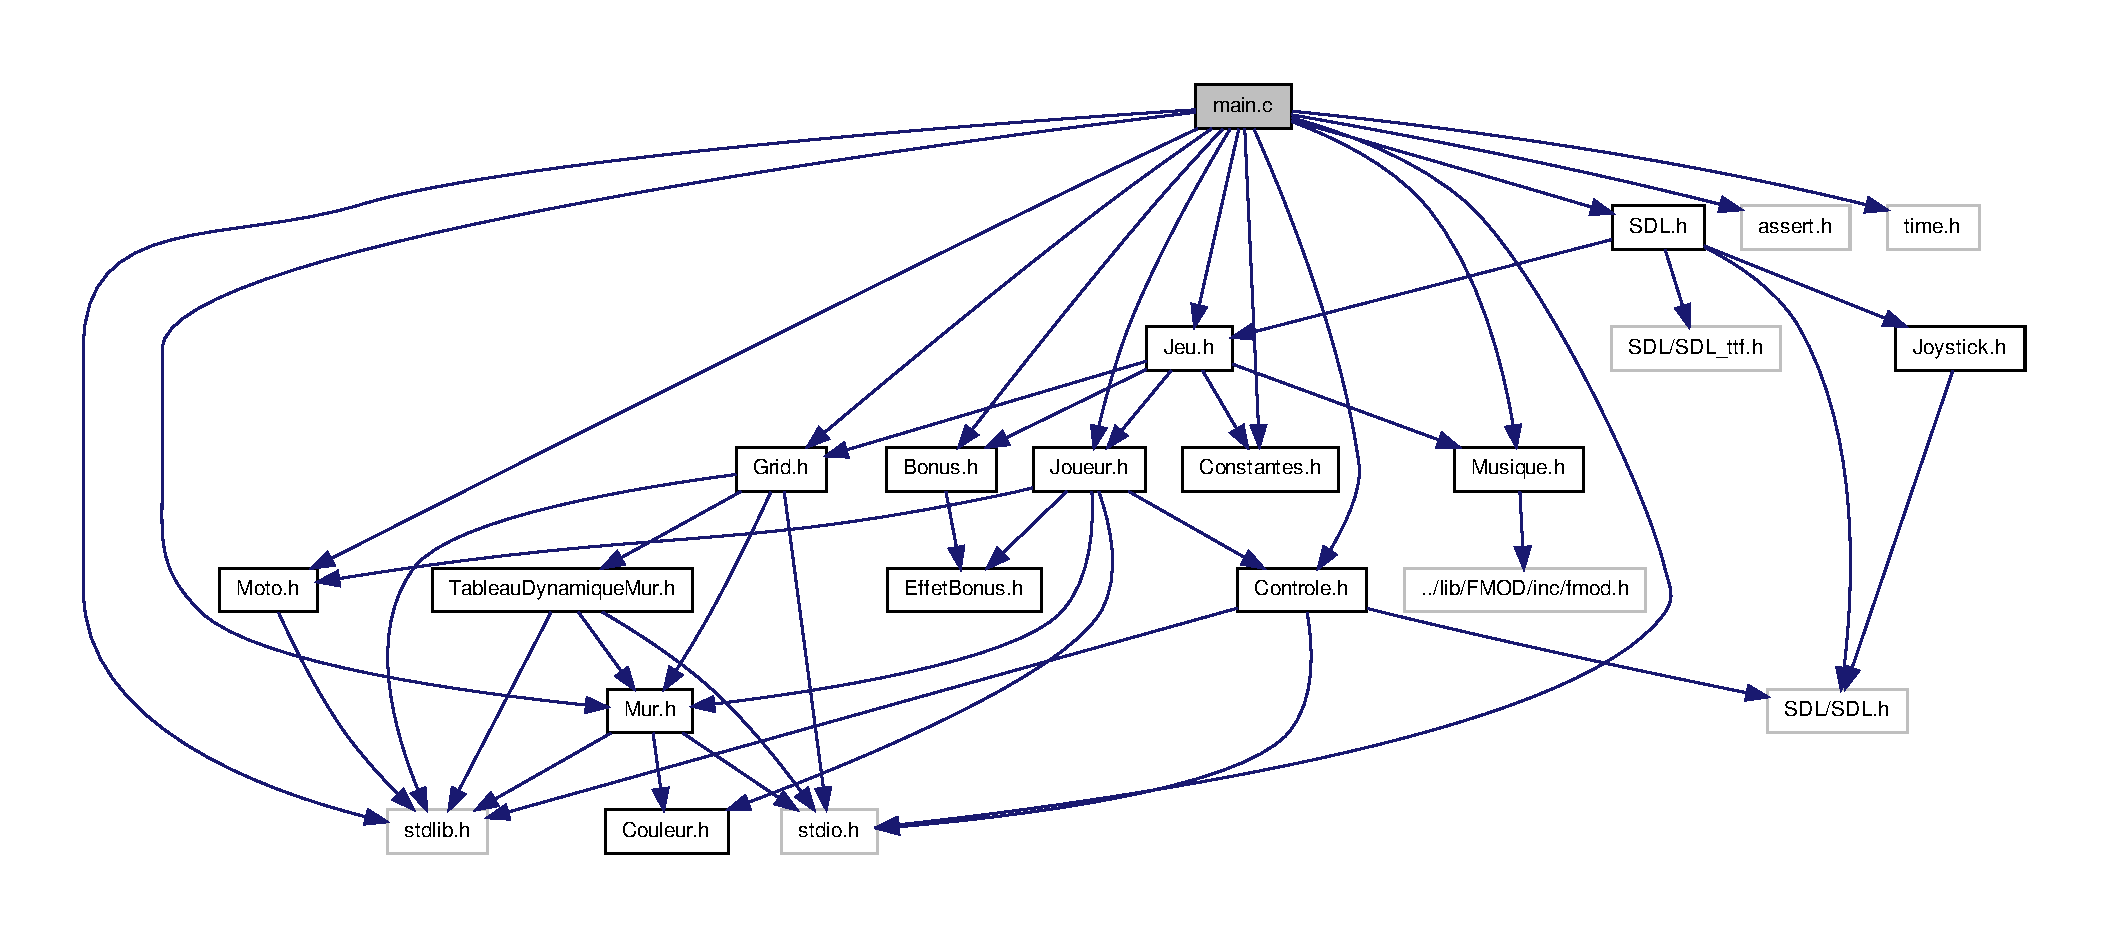
\includegraphics[width=350pt]{main_8c__incl}
\end{center}
\end{figure}
\subsection*{Fonctions}
\begin{DoxyCompactItemize}
\item 
int \hyperlink{main_8c_ae66f6b31b5ad750f1fe042a706a4e3d4}{main} ()
\end{DoxyCompactItemize}


\subsection{Description détaillée}
\hyperlink{main_8c}{main.\-c} \mbox{]} \begin{DoxyAuthor}{Auteur}
\{Antoine.\-C,Matthieu.\-B\} 
\end{DoxyAuthor}
\begin{DoxyVersion}{Version}
1.\-0 
\end{DoxyVersion}
\begin{DoxyDate}{Date}
13 mars 2013 
\end{DoxyDate}


Définition dans le fichier \hyperlink{main_8c_source}{main.\-c}.



\subsection{Documentation des fonctions}
\hypertarget{main_8c_ae66f6b31b5ad750f1fe042a706a4e3d4}{\index{main.\-c@{main.\-c}!main@{main}}
\index{main@{main}!main.c@{main.\-c}}
\subsubsection[{main}]{\setlength{\rightskip}{0pt plus 5cm}int main (
\begin{DoxyParamCaption}
{}
\end{DoxyParamCaption}
)}}\label{main_8c_ae66f6b31b5ad750f1fe042a706a4e3d4}


Définition à la ligne 24 du fichier main.\-c.


\hypertarget{pixel_8h}{\section{/home/antoine/\-L\-I\-F7\-\_\-td/src/pixel.h File Reference}
\label{pixel_8h}\index{/home/antoine/\-L\-I\-F7\-\_\-td/src/pixel.\-h@{/home/antoine/\-L\-I\-F7\-\_\-td/src/pixel.\-h}}
}
{\ttfamily \#include $<$stdlib.\-h$>$}\\*
{\ttfamily \#include $<$stdio.\-h$>$}\\*
\subsection*{Classes}
\begin{DoxyCompactItemize}
\item 
struct \hyperlink{structPixel}{Pixel}
\end{DoxyCompactItemize}

\printindex
\end{document}
